\documentclass[11pt,italian]{article}
\usepackage[T1]{fontenc}
\usepackage[utf8]{inputenc} %utf8 % lettere accentate da tastiera
\usepackage[italian]{babel} % lingua del documento
\usepackage{blindtext}
\usepackage{enumitem}
\usepackage{upquote}
\usepackage{float}
\usepackage{rotating}
\usepackage{xcolor}   % for \textcolor
\usepackage[font=small,labelfont=bf,skip=10pt]{caption}
\usepackage{subcaption}
\setlength{\belowcaptionskip}{5pt}
\usepackage{listings}
\lstset{
  basicstyle=\small\ttfamily,
  otherkeywords={self},             % Add keywords here
  basicstyle=\small\ttfamily,
  columns=fullflexible,
  frame=single,
  breaklines=true,
  postbreak=\mbox{\textcolor{red}{$\hookrightarrow$}\space},
  tabsize=4, % tab space width
  showstringspaces=false, % don't mark spaces in strings
  numbers=left, % display line numbers on the left
  commentstyle=\color[HTML]{a0a1a7}, % comment color
  keywordstyle=\color[HTML]{40a3f5}, % keyword color
  stringstyle=\color{red}, % string color,
  emphstyle={\color[HTML]{40a3f5}}
}
\usepackage{pythonhighlight}
\usepackage{hyperref}
\usepackage{cleveref}
\usepackage{graphicx}
\graphicspath{ {./images/} }

% Use lstinline as item in description
\makeatletter
\newcommand*{\lstitem}[1][]{%
  \setbox0\hbox\bgroup
    \patchcmd{\lst@InlineM}{\@empty}{\@empty\egroup\item[\usebox0]\leavevmode\ignorespaces}{}{}%
    \lstinline[#1]%
}
\makeatother

\title{Multiple Sequence Alignment (MSA) \\ di sequenze SARS-CoV-2}

\date{A.A.: 2019/2020}

\author{
    \textsc{Edoardo Silva} 816560 \\
    \textsc{Davide Marchetti} 815990
}

\begin{document}
\maketitle

\section{Abstract}
La seconda parte del progetto prevede di elaborare i file prodotti in precedenza ricavando informazioni relative alle alterazioni rilevate e producendo in output una tabella riassuntiva contenente:
\begin{itemize}
  \item il gene id del gene in cui cade la variazione con lo start e l'end della sua CDS rispetto alla reference
  \item il codone (o i codoni) alterato della reference, con posizione di inizio rispetto alla CDS, sequenza del codone e amminoacido codifcato
  \item il nuovo codone generato dalla variazione (o i nuovi codoni generati) specifcando la sequenza del codone e il nuovo amminoacido codifcato
\end{itemize}

\newpage
\section{Espressione genica}
I passi fondamentali per capire come un gene esprime una particolare proteina prevedono:
\begin{enumerate}
  \item Trascizione: sostituzione della Timina (T) con Uracile (U), ottenendo pre-mRNA
  \item Splicing: eliminazione delle sequenze introniche e concatenazione degli estroni per ottenere mRNA (oppure trascritto)
  \item Traduzione: traduzione in proteine dei \textbf{codoni} (triplette di basi) della CDS (sottostringa dell’mRNA)
\end{enumerate}

\noindent
Risulta triviale come un'alterazione della sequenza di DNA iniziale possa protrarsi fino alla fase di traduzione, andando ad alterare la produzione delle proteine di un particolare gene.

\vspace{1mm}
Attraverso le informazioni raccolte in questa fase saremo in grado di identificare in quali geni si concentrano le variazioni rilevate, dove queste avvengano e in che modo alterino i codoni e le rispettive proteine codificate.

\newpage
\section{Formato di output}
Ad ogni variazione analizzata corrisponde un entrata nella struttura dati a lista contenente le seguenti informazioni:
\begin{itemize}
    \item \lstinline{gene_id}: id del gene in cui cade la variazione
    \item \lstinline{gene_start}: inizio del gene in cui cade la variazione (1-based)
    \item \lstinline{gene_end}: fine del gene in cui cade la variazione (1-based)
    \item \lstinline{cds_start}: inizio della \lstinline{Coding DNA Sequence} della porzione del gene in cui cade la variazione (1-based)
    \item \lstinline{cds_end}: fine della \lstinline{Coding DNA Sequence} della porzione del gene in cui cade la variazione (1-based)
    \item \lstinline{relative_start}: inizio della variazione in rispetto all'inizio della cds (1-based)
    \item \lstinline{relative_end}: fine della variazione in rispetto all'inizio della cds (1-based)
    \item \lstinline{alteration}: sequenza della variazione
    \item \lstinline{original_codone}: codone della reference prima della modifica
    \item \lstinline{original_aminoacid}: amminoacido codificato da \lstinline{original_codone}
    \item \lstinline{altered_codone}: codone della reference modificati dalla variazione
    \item \lstinline{encoded_aminoacid}: amminoacido codificato da \lstinline{altered_codone}
\end{itemize}

\begin{sidewaysfigure}
  \makebox[\textwidth][c]{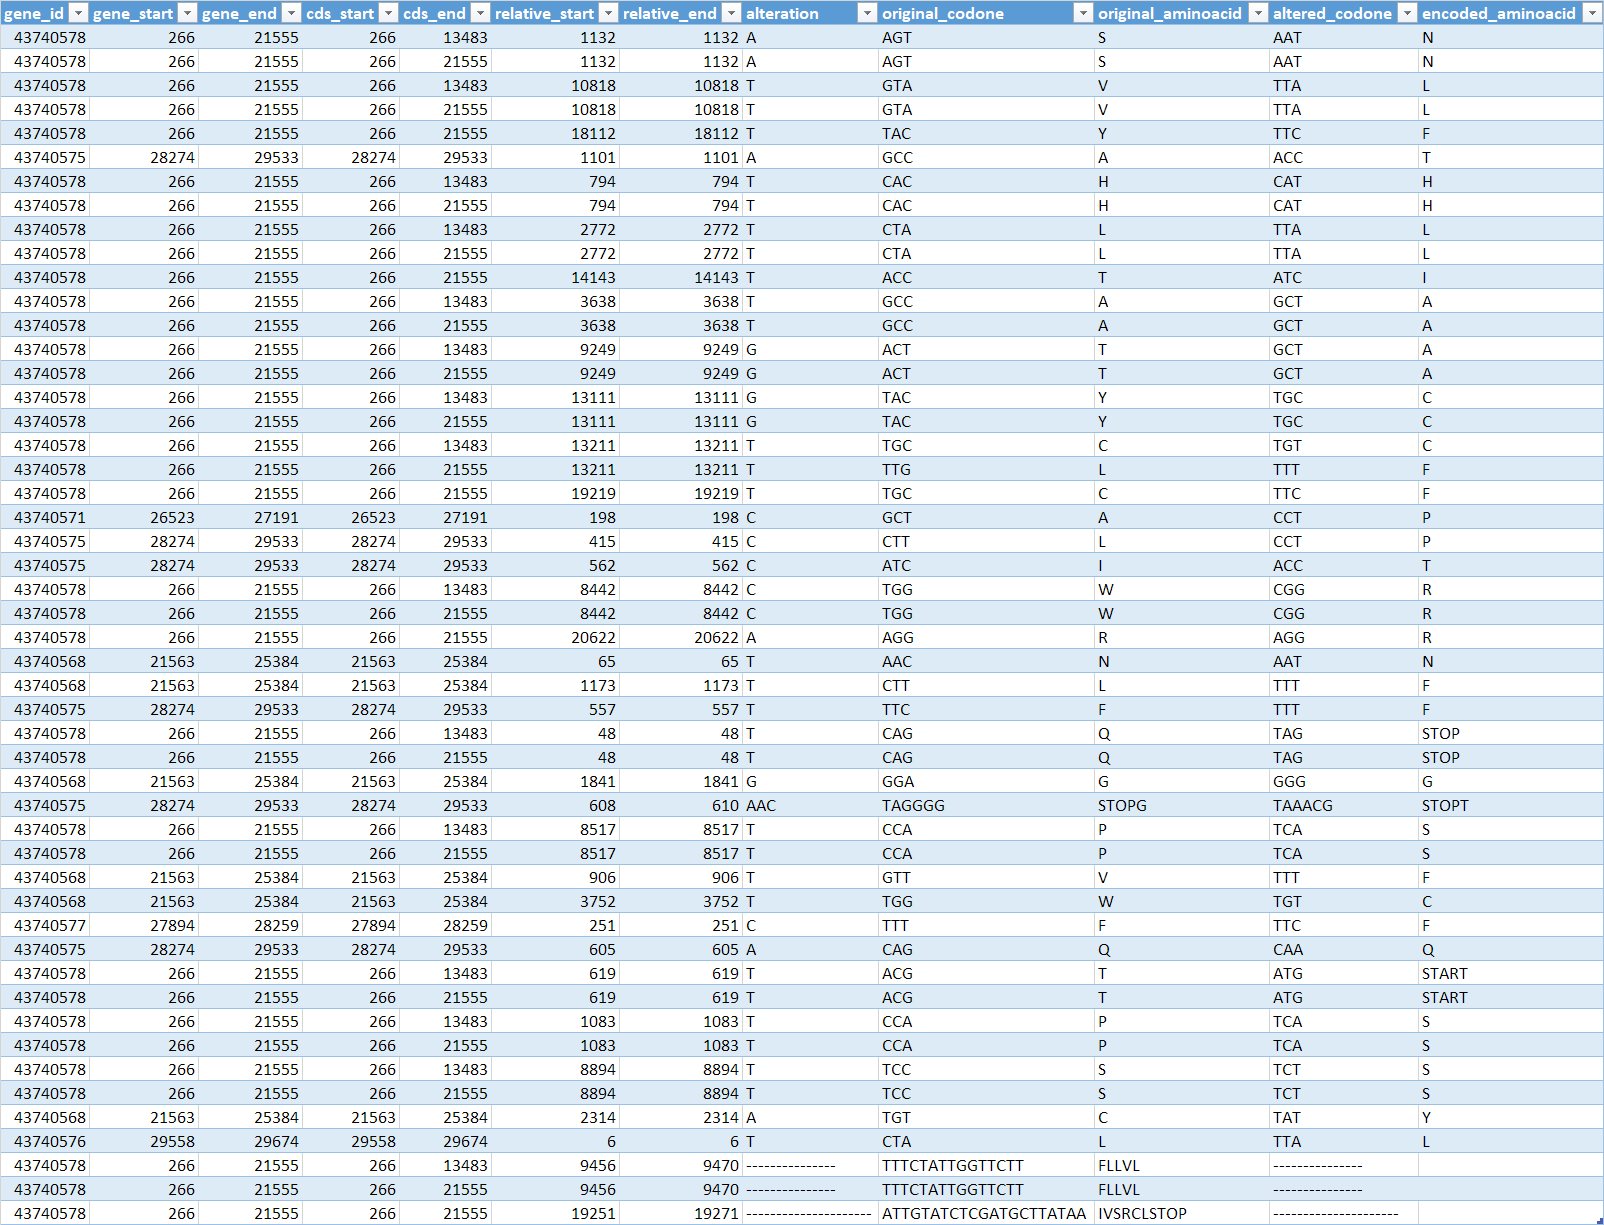
\includegraphics[width=1\linewidth]{alteration-table.png}}
  \caption{Tabella di output delle alterazioni}
  \label{fig:alteration_table}
\end{sidewaysfigure}

\newpage
\section{Algoritmo}
L'algoritmo inizia caricando tutti i file necessari per l'elaborazione, in particolare quelli prodotti in output nella parte precedente del progetto:
\begin{enumerate}
  \item Caricamento della sequenza reference dal fasta della sequenza di Wuhan \lstinline{NC_045512.2}.
  \item Caricamento di uno dei file di output prodotti nella prima parte di progetto. Nel nostro caso è stato utilizzata l'analisi dell'allineamento di \lstinline{ClustalW}.
  \item Lettura del file contenente le informazioni sui geni e le CDS della sequenza di riferimento. In particolare, una delle CDS analizzate derivava dall'unione (join) di due sequenze. In tal caso è possibile specificare il punto di unione della sequenza.
\end{enumerate}

\noindent
Dopo la lettura del materiale rilevante a questa fase di elaborazione, l'algoritmo itera le variazioni rilevate nell'allineamento e per ciascuna di esse esegue i seguenti step:
\begin{enumerate}
  \item Identifica le CDS nelle quali avviene l'alterazione rispetto alla sequenza reference.
  \item Effettua una sostituzione della \lstinline{Timina} (\lstinline{T}) con l'\lstinline{Uracile} (\lstinline{U}) nelle sezioni coinvolte delle sequenze.
  \item Recupera le informazioni del gene associato alle CDS rilevate calcolando le posizioni globali e relative alla CDS dell'alterazione.
  \item Identifica i codoni alterati e ne effettua la ritraduzione in amminoacidi grazie ad una look-up table (listato \ref{code:aminoacids_table}). Vengono ignorate le alterazioni che presentano sequenze di soli \lstinline{-}, derivate probabilmente da un sequenziamento errato o un'alterazione posta ai capi dell'allineamento.
  \item Memorizza tutte le informazioni ricavate in una struttura dati apposita tramite cui derivare la tabella per l'output finale associando i valori a chiavi prestabilite.
\end{enumerate}

\noindent
La struttura dati così ottenuta sarà esportata in formato CSV per permettere una visualizzazione agevolata attraverso programmi terzi (come riportato in \cref{fig:alteration_table}).

\newpage
\section{Analisi dei risultati e conclusioni}
Come riportato in \cref{fig:alteration_table} la maggior parte delle alterazioni coinvolgono un singolo codone e, anche nel caso di cancellazioni, la CDS risultante rimane traducibile (rimane multipla di tre). In alcuni casi, l'amminoacido risultante dalla traduzione dell'alterazione non viene modificato.

Le ultime righe della tabella riportano delle alterazioni che determinano la cacellazione di alcune basi rispetto alla sequenza reference.
Queste sono relative esclusivamente alla sola sequenza \lstinline{MT262993.1} e si pensa possano derivare da un errore in fase di sequenziamento.

\subsection{Distribuzione delle variazioni all'interno delle CDS}
Rispetto alle variazioni identificate ed analizzate, più del 65\% risultano appartenenti ad almeno una CDS e riportate in tabella.
\begin{figure}[H]
  \makebox[\textwidth][c]{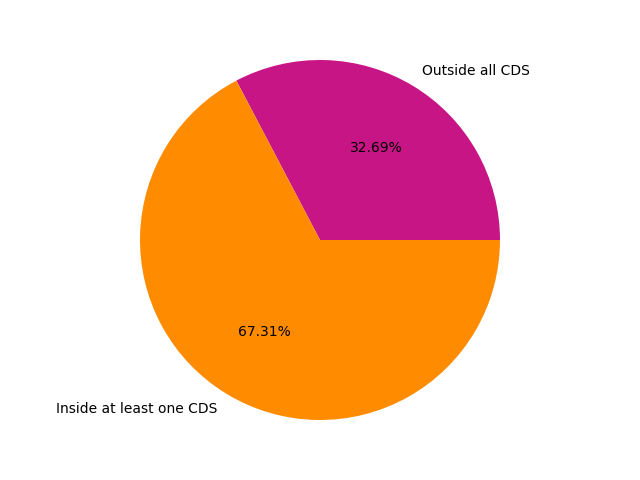
\includegraphics[width=0.6\linewidth]{plot-alteration-in-cds.png}}
  \caption{Percentuale di variazioni interne ed esterne alle CDS}
  \label{fig:plot-alterations-in-cds}
\end{figure}

Analizzando la distribuzione delle alterazioni che coinvolgono geni riportata in \cref{fig:plot-alterations-per-gene}, quasi i tre quarti del numero totale di variazioni si concentrano nel gene \lstinline{ORF1ab}. Questo era un risultato atteso, essendo un gene composto da più di 21.000 basi.

\vspace{1mm}
Infine, dal grafico delle alterazioni appartenenti ad una CDS divise per sequenza (\cref{fig:plot-per-sequence}) notiamo una distribuzione piuttosto omogenea, eccetto per le sequenze \lstinline{MT262993.1} e \lstinline{MT276597.1} dove abbiamo un basso numero di alterazioni.
Al contrario, la sequenza nella quale si manifestano più alterazioni nelle CDS risulta essere \lstinline{EPI_ISL_437334}, che anche nelle analisi precedenti risultava avere il maggior numero di sostituzioni rispetto alle altre sequenze.
\begin{figure}[]
  \makebox[\textwidth][c]{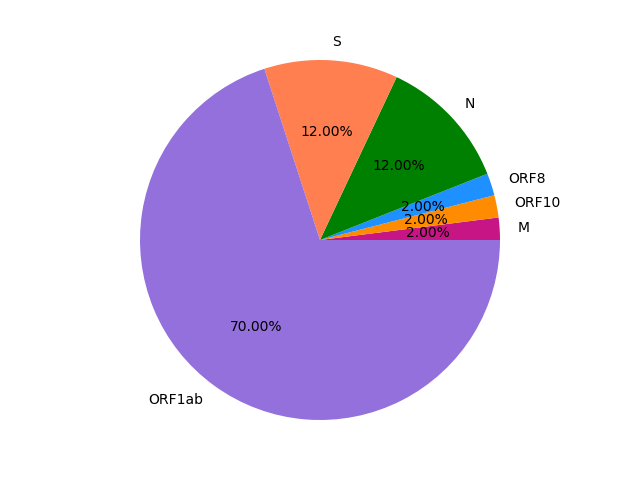
\includegraphics[width=0.8\linewidth]{plot-variations-per-gene.png}}
  \caption{Percentuale di variazioni per gene}
  \label{fig:plot-alterations-per-gene}
\end{figure}

\begin{figure}[H]
  \makebox[\textwidth][c]{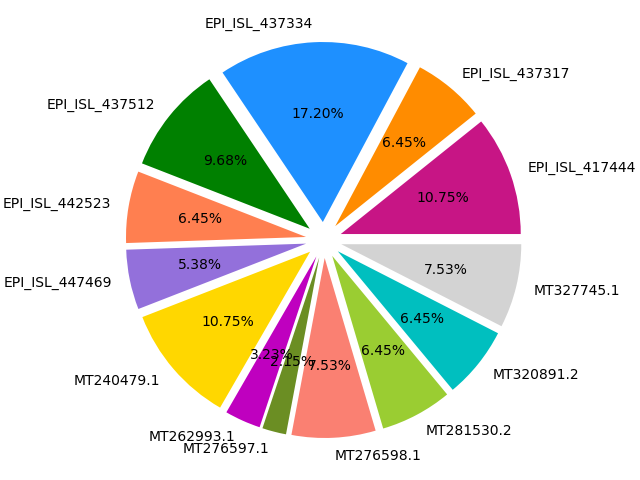
\includegraphics[width=0.8\linewidth]{plot-alteration-in-gene-per-sequence.png}}
  \caption{Tipologia di variazioni}
  \label{fig:plot-per-sequence}
\end{figure}

\subsection{Divisone del lavoro}
Durante la realizzazione del progetto entrambi i componenti del gruppo hanno partecipato attivamente alla sua realizzazione. In particolare:
\begin{itemize}
  \item \textbf{Edoardo Silva} si è occupato principalmente di recuperare e gestire l'output JSON del progetto1 e delle funzioni di supporto.
  \item \textbf{Davide Marchetti} si è occupato principalmente di generare i file di output e correggere le porzioni di codice relative alle letture delle reference.
  \item Entrambi hanno lavorato alla creazione ed elaborazione dei dati, alla matrice delle mutazioni e le traduzioni di quest'ultime.
\end{itemize}

\newpage
\section{Listati di codice}
\begin{lstlisting}[language=Python,caption=Tabella per la traduzione in amminoacidi,label=code:aminoacids_table]
aminoacids_lookup_table = {
  'F': ['UUU', 'UUC'],
  'L': ['UUA', 'UUG', 'CUU', 'CUA', 'CUC', 'CUG'],
  'I': ['AUU', 'AUC', 'AUA'],
  'M': ['AUG'],
  'V': ['GUU', 'GUA', 'GUC', 'GUG'],
  'S': ['UCU', 'UCA', 'UCC', 'UCG', 'AGU', 'AGC'],
  'P': ['CCU', 'CCA', 'CCC', 'CCG'],
  'T': ['ACU', 'ACA', 'ACC', 'ACG'],
  'A': ['GCU', 'GCA', 'GCC', 'GCG'],
  'Y': ['UAU', 'UAC'],
  'H': ['CAU', 'CAC'],
  'Q': ['CAA', 'CAG'],
  'N': ['AAU', 'AAC'],
  'K': ['AAA', 'AAG'],
  'D': ['GAU', 'GAC'],
  'E': ['GAA', 'GAG'],
  'C': ['UGU', 'UGC'],
  'W': ['UGG'],
  'R': ['CGU', 'CGA', 'CGC', 'CGG', 'AGA', 'AGG'],
  'G': ['GGU', 'GGA', 'GGC', 'GGG'],
  'STOP': ['UAA', 'UAG', 'TGA']
}
\end{lstlisting}

\end{document}